\section{Durchführung}
\label{sec:Durchführung}

\subsection{Effektiver Dämpfungswiderstand}
    Zunnächst wird mit dem in Abbildung \ref{fig:5a} gezeigten Stromkreis
    die Zeitabhängigkeit der Amplitude eines gedämpften Schwingkreises 
    untersucht.\\
    \begin{figure}
        \centering
        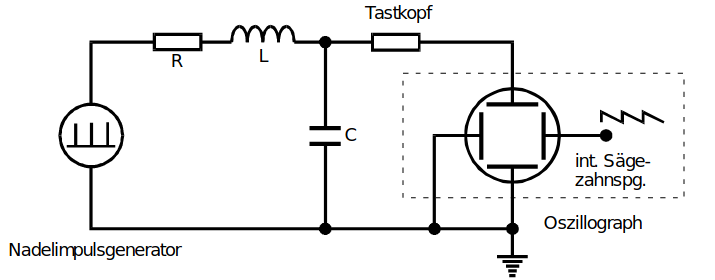
\includegraphics[width=0.75\textwidth]{5a.png}
        \caption{Versuchsaufbau zur Untersuchung der Amplitude.\cite{anleitung}}
        \label{fig:5a}
    \end{figure}

    \noindent Um den Schwingkreis zu erregen genügt ein kurzer Puls des 
    Nadelimpulsgenerators. Dabei hat die Amplitude zwischen zwei Pulsen 
    ausreichend Zeit, um den Faktor %3 bis 8
    abzuklingen.\\
    Da der Oszillograph, der zum betrachten der Schwingung verwendet wird,
    einen Eingangswiderstand hat, der eine zusätzliche dämpfende Wirkung
    auf das System hat, wird ein Tastkopf mit großem Widerstand $R = 10 \si{\mega\ohm}$
    eingebaut. Durch ihn wird der Einfluss des Oszillographen bis auf einen
    vernachlässigbar kleinen Teil verringert. 

\subsection{Dämpfungswiderstand beim aperiodischen Grenzfall}
    Des Weiteren wird das Verhalten des Schwingkreises bei aperiodischer 
    Schwingung genauer betrachtet. Dazu wird die Schaltung \ref{fig:5b} 
    verwendet.\\

    \begin{figure}
        \centering
        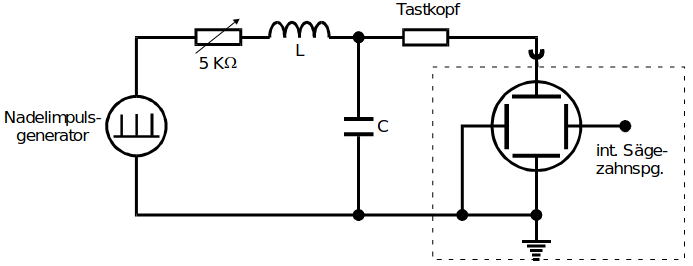
\includegraphics[width=0.75\textwidth]{5b.png}
        \caption{Versuchsaufbau zur Untersuchung des aperiodischen Grenzfalls.\cite{anleitung}}
        \label{fig:5b}
    \end{figure}

    \noindent Zu Beginn wird der regelbare Widerstand auf den Maximalwert eingestellt,
    dann langsam verringert. Es wird der Wert ermittelt, in dem gerade kein 
    Überschwingen auftritt.

\subsection{Frequenzabhängigkeit im Serienresonanzkreis}
    Es gilt zudem, im Serienresonanzkreis, der in Abbildung \ref{fig:5c} zu
    sehen ist, die Frequenzabhängigkeit der Kondensatorspannung zu messen.

    \begin{figure}
        \centering
        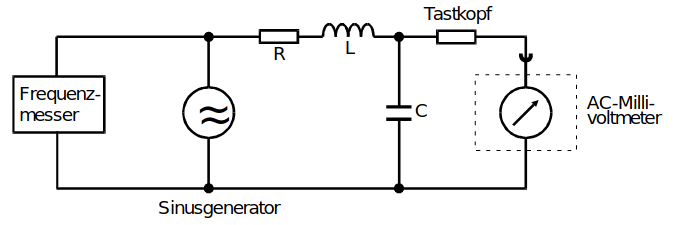
\includegraphics[width=0.75\textwidth]{5c.png}
        \caption{Serienresonanzkreis zur Untersuchung der Frequenz.\cite{anleitung}}
        \label{fig:5c}
    \end{figure}

    \noindent Wie zuvor hindert ein Tastkopf den Einfluss des Messgerätes, hier des Millivoltmeters, daran,
    zu groß zu werden. Da dessen Ausgangsspannung aber nicht unabhängig 
    vom der Frequenz ist, muss zur Korrektur auch die Erregerspannung über
    den Tastkopf gemessen werden. \\
    Der Innenwiderstand des Sinusgenerators muss auch betrachtet werden.

\subsection{Frequenzabhängigkeit der Phase}
    Um die Frequenzabhängigkeit der Phase zwischen Erreger- und
    Kondensatorspannung zu messen, wird die Anordnung in 
    \ref{fig:5d} genutzt.

    \begin{figure}
        \centering
        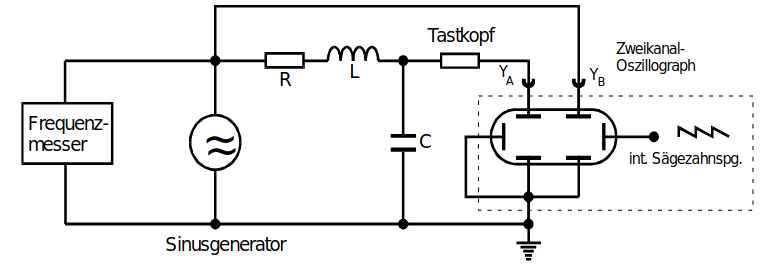
\includegraphics[width=0.75\textwidth]{5d.png}
        \caption{Messung der Frequenzabhängigkeit der Phase.\cite{anleitung}}
        \label{fig:5d}
    \end{figure}

    \noindent Es wird ein Zweistrahl-Oszilloskop verwendet, in das die 
    Kondensatorspannung und die Erregerspannung gegeben werden. 
    Für eine Phase $\phi > 0$ erhält man eine Anzeige wie in Abbildung
    \ref{fig:verschiebung}. Es ist dabei wichtig, dass beide Sinuskurven
    so eingestellt sind, dass sie symmetrisch zur x-Achse liegen.

    \begin{figure}
        \centering
        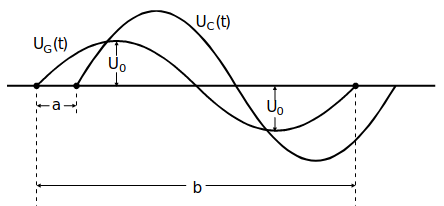
\includegraphics[width=0.75\textwidth]{5d2.png}
        \caption{Anzeige eines Zweistrahloszillographen zur Messung der Phasenverschiebung. \cite{analt}}
        \label{fig:verschiebung}
    \end{figure}

\subsection{Scheinwiderstand}
    Zuletzt wird der Scheinwiderstand des Serienresonanzkreises durch 
    Messung von Generatorspanung und Strom errechnet. Die dazu verwendete
    Schaltung ist in Abbildung \ref{fig:5e} gezeigt.

    \begin{figure}
        \centering
        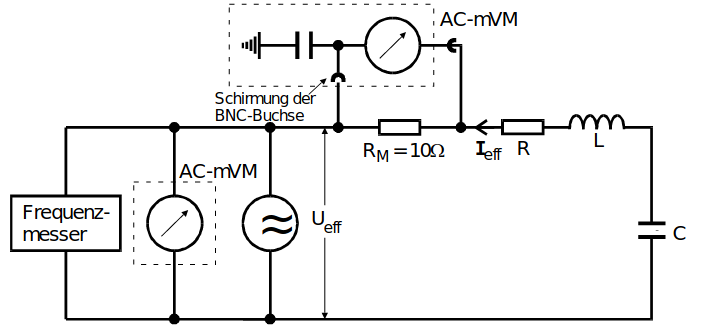
\includegraphics[width=0.75\textwidth]{5e.png}
        \caption{Schaltung zur Messung des Scheinwiderstandes.\cite{anleitung}}
        \label{fig:5e}
    \end{figure}

    \noindent Anstelle eines Amperemeters wird zur Messung des hochfrequenten 
    Stroms ein geringer Widerstand verwendet, sodass an ihm ein Spannungsabfall 
    festgestellt werden kann. Das dazu genutzte Millivoltmeter wird am Sinusgenerator
    geerdet. \\
    Eine weitere Möglichkeit, den Scheinwiderstand zu messen, ist mit einem Impedanzmeter.
    Die dazu nötige Schaltung ist in Abbildung \ref{fig:5e2} zu sehen.

    \begin{figure}
        \centering
        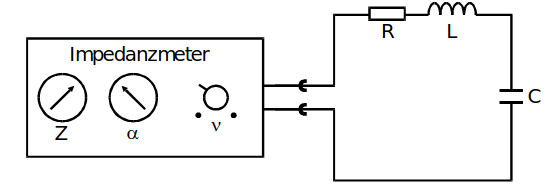
\includegraphics[width=0.75\textwidth]{5e2.png}
        \caption{Messung des Scheinwiderstandes mit Impedanzmeter.\cite{anleitung}}
        \label{fig:5e2}
    \end{figure}
